\documentclass[a4paper]{article}     
\usepackage{amsfonts}
\usepackage{amsmath}
\usepackage{amssymb}
\usepackage{graphicx}


\begin{document}

\noindent \large Auteur: Xander De Blauwer \\
\noindent \large Studierichting: Informatica\\
\noindent \large Oefeningenreeks 5D nr. 2.2\\

\medskip

\normalsize


$f(x) = e^x $ op $[0,1]$ en $[-2,2]$ \\

$[0,1]: \displaystyle\int_{0}^{1} e^x dx = \left[ e^x \right]_{0}^{1} = e - 1 $ \\

$[-2,2]: \displaystyle\int_{-2}^{2} e^x dx = \left[ e^x \right]_{-2}^{2} = e^2 - \dfrac{1}{e^2} $ \\

\begin{figure}[h]
\centering
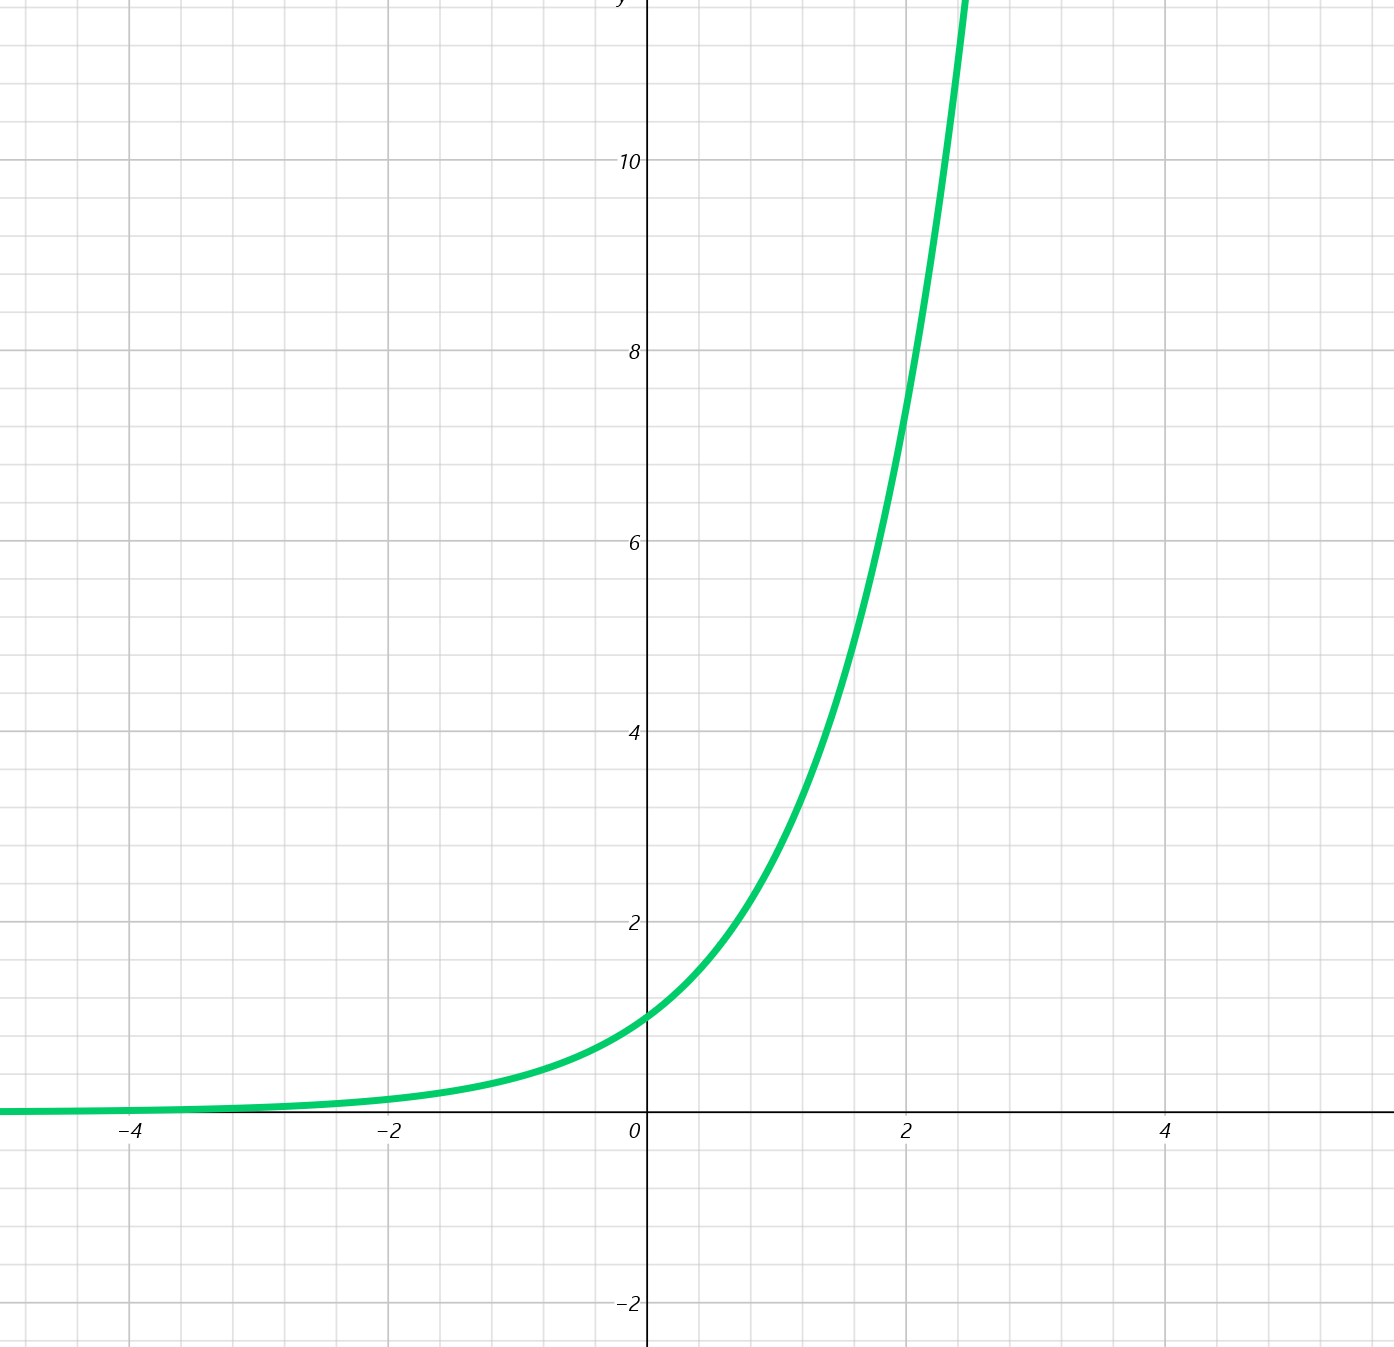
\includegraphics[width=5cm]{5D-2.2-xander.de.blauwer.INF.png}
\end{figure}



\begin{thebibliography}{999}
%\bibitem{a} Referentie
\end{thebibliography}
\end{document} 